\chapter{\IfLanguageName{dutch}{Proof of concept}{Proof of concept}}%
\label{ch:proofofconcept}

Dit hoofdstuk beschrijft eerst welke technologieën gebruik zijn voor het ontwikkelen van Move-it. Daarna wordt de opbouw van de webapplicatie besproken en geïllustreerd met schermafbeeldingen.

\section{Gekozen technologieën}

\subsection{Framework}

Gezien de expertise van \href{https://www.we-are.be/}{we are}, is er voor het platform gekozen voor een responsive React\footnote{\href{https://react.dev/}{https://react.dev/}}-website. Hiervoor is gebruik gemaakt van TypeScript \footnote{\href{https://www.typescriptlang.org/}{https://www.typescriptlang.org/}}.

Voor de implementatie van authenticatie is er gebruik gemaakt van Auth0\footnote{\href{https://auth0.com/}{https://auth0.com/}}. De redenen waarom er voor Auth0 gekozen is, zijn: de mogelijkheid om aan te melden met een Google-account, makkelijke integratie in React en de mogelijkheid tot een gratis abonnement wanneer het aantal gebruikers onder de 7000 blijft, wat voor deze POC meer dan voldoende is.

\subsection{Component libraries}
Gezien de korte ontwikkeltijd die beschikbaar was, zijn Material UI Core\footnote{\href{https://mui.com/core/}{https://mui.com/core/}} en Material UI X\footnote{\href{https://mui.com/x/}{https://mui.com/x/}} component libraries gebruikt voor de ontwikkeling van deze website, om zo het ontwikkelproces te vergemakkelijken. Er is gekozen voor Material UI wegens diens universele look-and-feel, het ruime aanbod aan gratis componenten en de beschikbaarheid van verschillende grafiek-componenten. Daarnaast zijn deze componenten uitermate geschikt voor zowel mobiel als desktop gebruik, wat de ``User Experience'' (UX) verbetert.

\subsection{Databank}

Deze applicatie gebruikt een graafdatabank, meer specifiek Neo4J\footnote{\href{https://neo4j.com/}{https://neo4j.com/}}. Er is in deze situatie gekozen voor een graaf databank omdat het zeer simpel op te zetten is en er geen databank-schema ontworpen moet worden, wat er dus voor zorgt dat het mogelijk is om snel te ontwikkelen en gaandeweg eventueel zaken aan te passen indien nodig.

Daarnaast zal de analyse van de ingegeven sportdata ook makkelijker verlopen: er zullen geen complexe join-operaties aan te pas komen om bijvoorbeeld alle activiteiten van de deelnemers van een team op te vragen, wat bij een SQL-databank wel het geval zou zijn.

\subsection{Deployment}

De website wordt gedeployed met behulp van Vercel\footnote{\href{https://vercel.com/home}{https://vercel.com/home}}. De GitHub\footnote{\href{https://github.com/}{https://github.com/}}-repository van deze applicatie is gelinkt aan een Vercel-project, wat er voor zorgt dat de elke nieuwe commit op de main-branch steeds gedeployed zal worden. Dit maakt het zeer eenvoudig om te beheren. Move-it is terug te vinden op \href{https://move-it-ghent.vercel.app/}{https://move-it-ghent.vercel.app/}.

\section{Opbouw van de applicatie}

De applicatie is opgesteld op basis van de volgende bouwstenen: een centraal dashboard, een overzicht van eigen prestaties, een oplijsting van de teamleden en een profielpagina.

\subsection{Dashboard}
Op het dashboard is de meeste informatie te zien: zowel persoonlijke evolutie over één week en een overzicht van het type uitgevoerde activiteiten (figuur \ref{fig:graphs}) als de team en persoonlijke ranking (figuur \ref{fig:personalRanking} en \ref{fig:teamRanking}) zijn er te vinden. Om kleinere teams evenveel kans te geven, houdt de teamranking rekening met de grote van het team bij de berekening.

\begin{figure}[h]
    \caption[Team ranking]{De team ranking, gezien vanop een laptop.}
    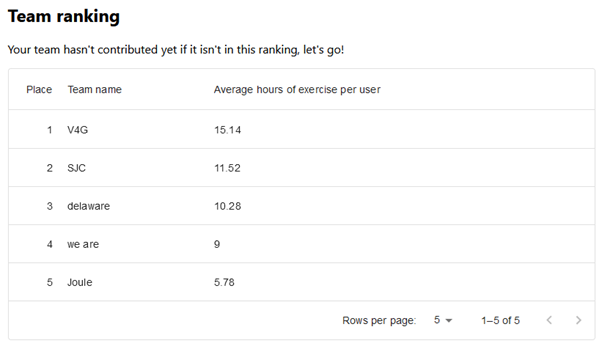
\includegraphics[width=1\textwidth]{TeamRanking}
    \label{fig:teamRanking}
\end{figure}

\begin{figure}[h]
    \caption[Persoonlijke ranking]{De persoonlijke ranking, gezien vanop een laptop.}
    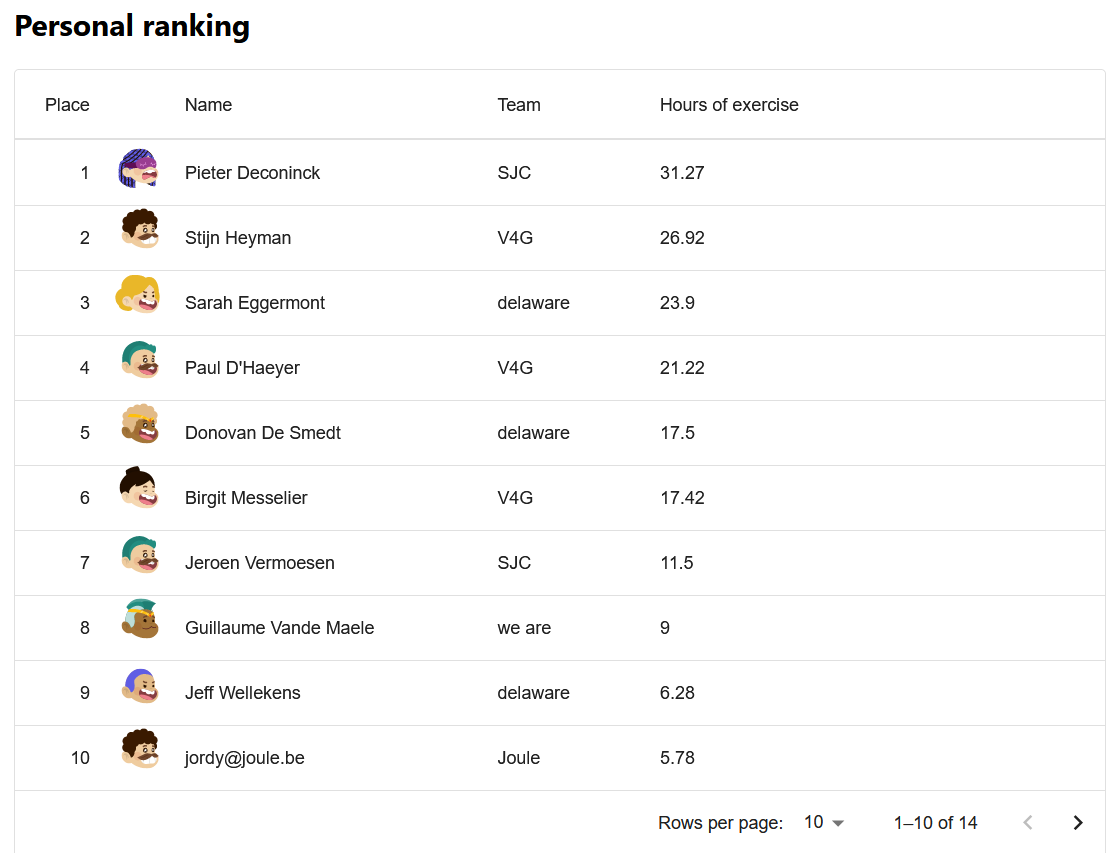
\includegraphics[width=1\textwidth]{PersonalRanking}
    \label{fig:personalRanking}
\end{figure}

Op het dashboard is vooral ingezet op scoreborden en het visualiseren van persoonlijke vooruitgang. De punten zijn hier in de vorm van gepresteerde uren weergegeven. Door persoonlijke vooruitgang in een grafiek te tonen, kan een gebruiker gestimuleerd worden om zichzelf steeds te proberen overtreffen door de lijn van de linkse grafiek naar boven te laten wijzen.

\begin{figure}[h]
    \caption[Overzicht prestaties dashboard website]{Overzicht van gepresteerde uren de afgelopen week en van het type activiteiten sinds de lancering van de applicatie, gezien vanop een laptop.}
    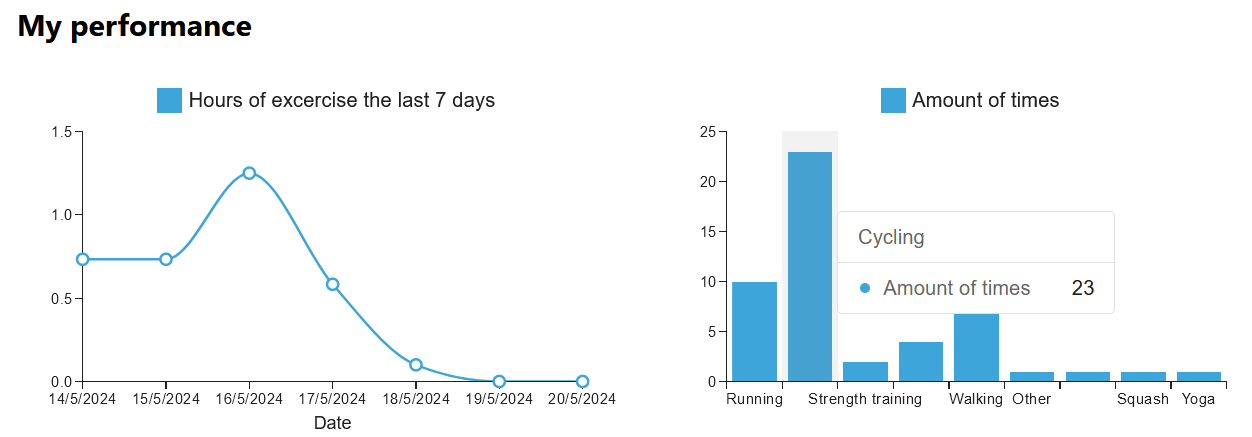
\includegraphics[width=1\textwidth]{MyGraphs}
    \label{fig:graphs}
\end{figure}

\subsection{Persoonlijk overzicht}
Op het persoonlijk overzicht is een lijst van de gepresteerde activiteiten te zien (figuur \ref{fig:performances} en figuur \ref{fig:performancesMobile}), en kunnen gebruikers ook hun prestaties ingeven. Hier is voldoende ruimte voorzien voor de ingave van technische gegevens, zoals gemiddelde hartslag en hoogtemeters. Afhankelijk van het type activiteit, en wanneer een afstand en duur ingegeven zijn, berekent de applicatie ook een gemiddelde snelheid. Zo kunnen frequente sporters eventueel een vooruitgang opmerken.

\begin{figure}[h]
    \caption[Overzicht activiteiten website]{Overzicht van gepresteerde activiteiten in de applicatie, gezien vanop een laptop.}
    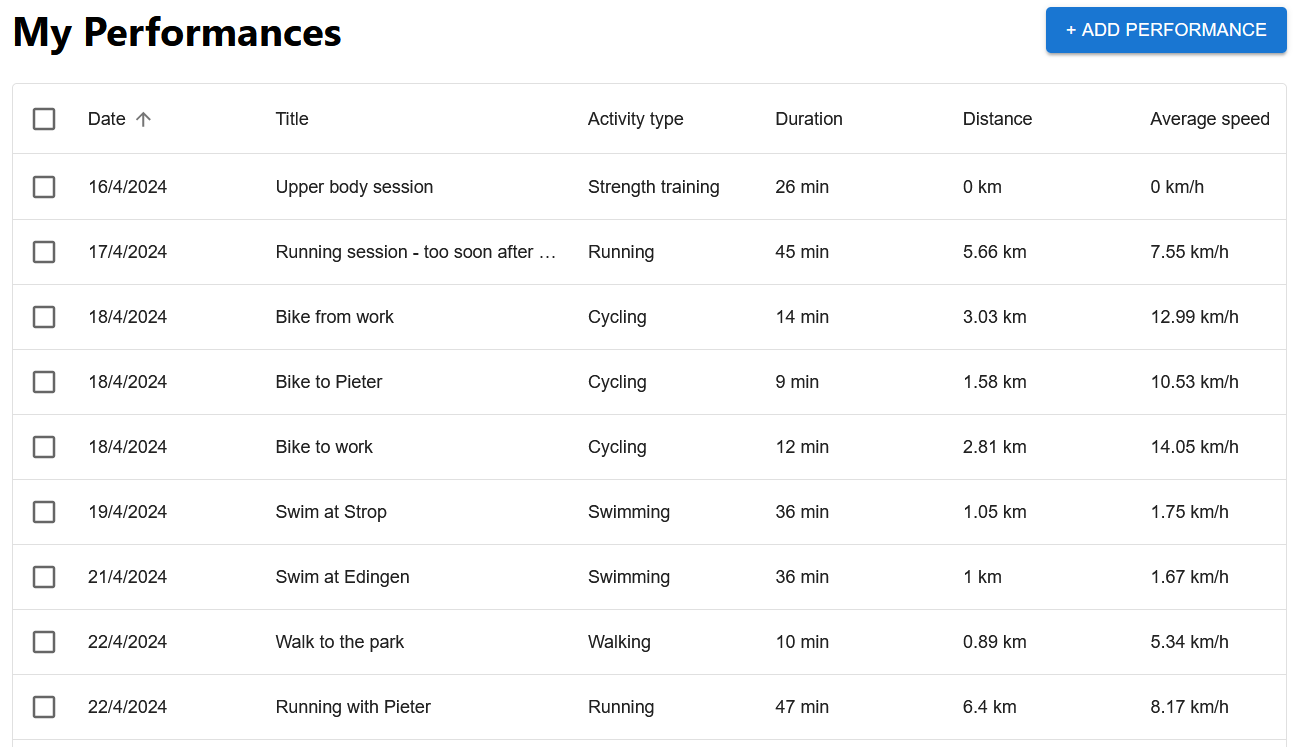
\includegraphics[width=1\textwidth]{MyPerformances}
    \label{fig:performances}
\end{figure}

\begin{figure}[h]
    \caption[Overzicht activiteiten website smartphone]{Overzicht van gepresteerde activiteiten in de applicatie, gezien vanop een smartphone.}
    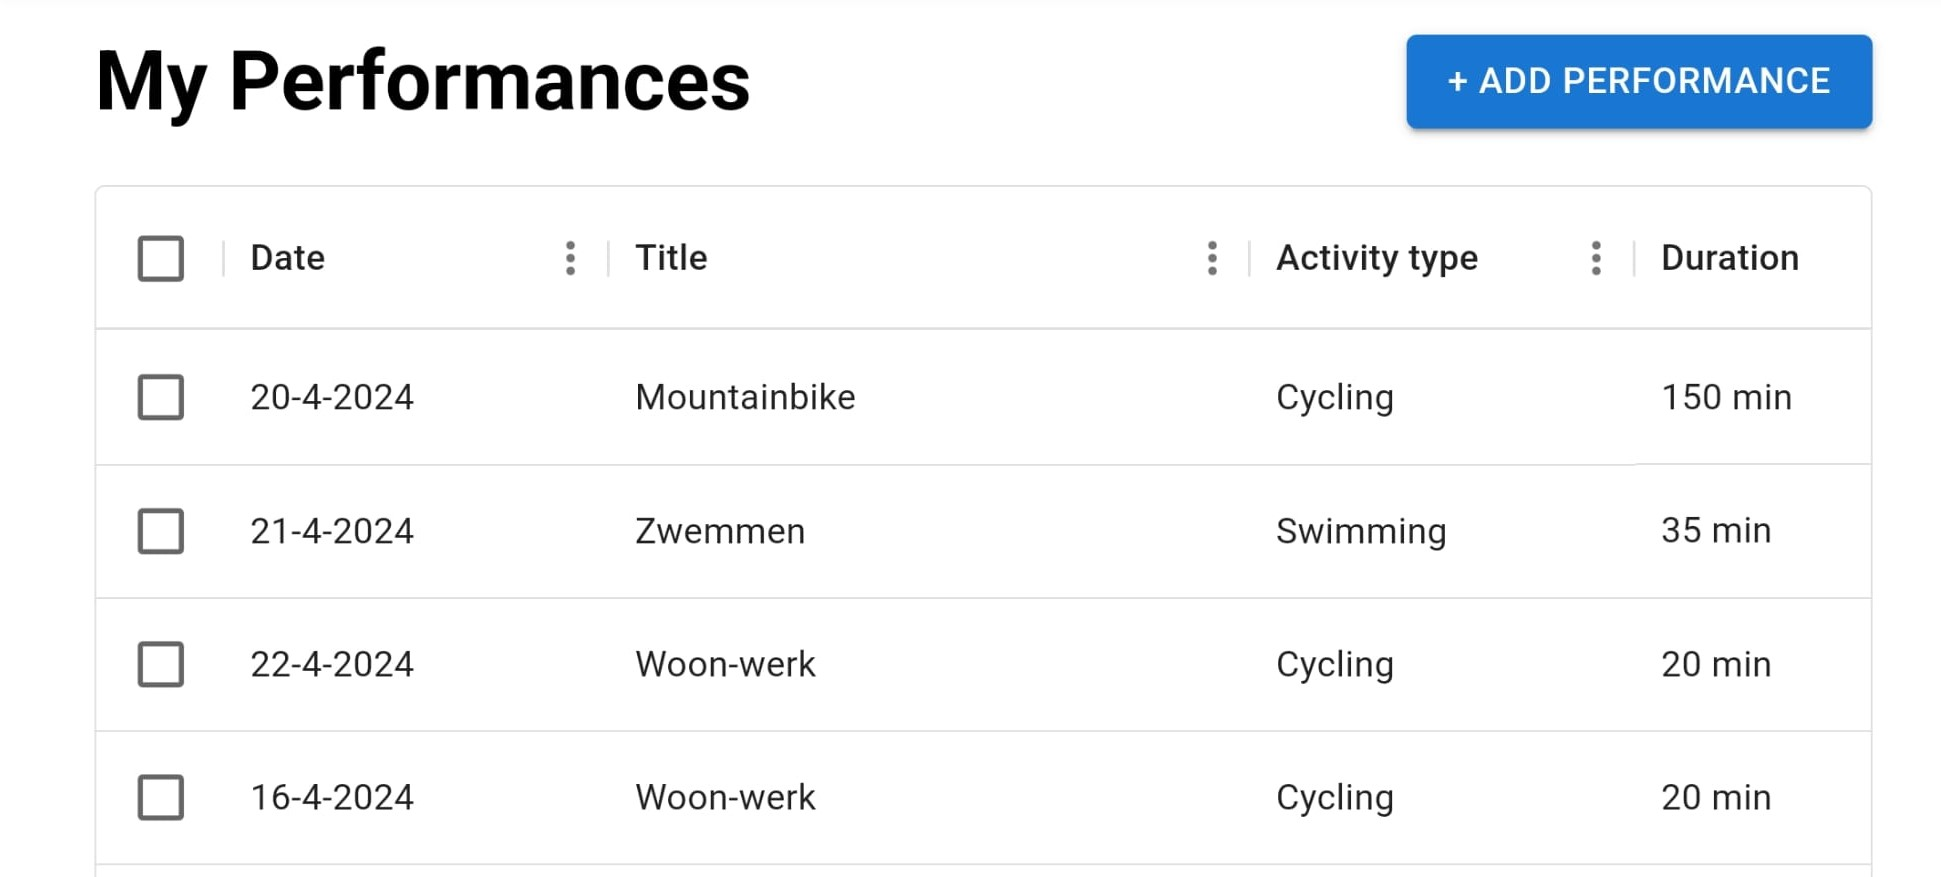
\includegraphics[width=1\textwidth]{MyPerformancesMobile}
    \label{fig:performancesMobile}
\end{figure}

\subsection{Teamoverzicht}

Dit overzicht is een simpele oplijsting van alle teamleden waartoe de aangemelde gebruiker behoort (figuur \ref{fig:team}).

In de toekomst zou dit uitgebreid kunnen worden met een overzicht van de prestaties van een team, zodat er ook binnen een team gamification speelt, wat mogelijks tot nog meer motivatie kan leiden.

\begin{figure}[h]
    \caption[Overzicht van teamleden]{Overzicht van teamleden in de applicatie, gezien vanop een laptop. Mailadressen zijn wazig gemaakt om privacy-redenen.}
    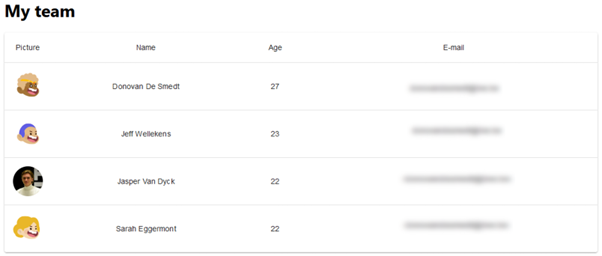
\includegraphics[width=1\textwidth]{MyTeam}
    \label{fig:team}
\end{figure}

\subsection{Profiel pagina}

Op deze pagina kan een gebruiker een avatar, team en naam kiezen waarmee die weergegeven wordt.